\documentclass{article}

\usepackage[T1]{fontenc}
\usepackage[utf8]{inputenc}
\usepackage[spanish]{babel}
\usepackage{graphicx}
\usepackage{microtype}
\usepackage{xcolor}
\usepackage{amsmath}
\usepackage{booktabs}
\usepackage{hyperref}
\usepackage{siunitx}

\newcommand{\todox}{\(\mathit{\color{red}x}\)}
\newcommand{\ham}{\large{\texttt{ham}}}
\newcommand{\spam}{\large{\texttt{spam}}}
\newcommand{\fo}{\(\mathbf{F_1}\)}

\interfootnotelinepenalty=10000

\title{Aprendizaje Automático \\ Trabajo Práctico 1 --- Detección de Spam}
\author{Martín Fixman \and Leandro Matayoshi \and Fernando Gasperi}
\date{Segundo Cuatrimestre de 2016}

\begin{document}
\maketitle

\newpage

\section{Introducción}

En este trabajo se midel diferentes basado en técnicas de \textbf{Apredizaje Automático} para clasificación de mails entre \ham{} o \spam{}.

La entrada consiste de \num{45000} mensajes clasificados a priori como \ham{}, y otros \num{45000} clasificados a priori como \spam{}. Para ayudar a medir las inferencias, tomamos el 10\% de cada uno de estos (\num{4500} \ham{} y \num{4500} \spam{}) como \textit{testing set}, y no hacemos ningún experimento sobre estos hasta el final del trabajo, cuando se miden los modelos. 

\section{Extracción de Atributos}

\subsection{Análisis de texto}

Para obtener atributos relacionados con análisis de texto decidimos trabajar específicamente con 2 campos: \(body\) y \(subject\).

La extracción se realizó en base a aplicar Bayes sobre la probabilidad de que un mensaje sea \spam{} dada la aparición de una palabra (potencial atributo) en dicho mensaje.

Sea $w \in W$, siendo $W$ el universo de palabras obtenido a partir de los mails utilizados para entrenar el modelo.

\vspace{5px}
$P(spam \vert w) = \frac{P(w \vert spam) \cdot P(spam)}{P(w)}$, donde:

\vspace{5px}
$P(w \vert spam) = \frac{\sum_{s \in spam}^{} w \in s}{\mid spam \mid}$, $P(w) = \frac{\sum_{m \in M}^{} w \in m}{\mid M \mid}$, $P(spam) = \frac{\mid spam \mid}{\mid M \mid}$

\vspace{5px}
Análogamente, se realiza la misma operación para analizar las palabras que aparecen en los mails de \ham{}.

El primer experimento consistió en encontrar las 100 palabras que aparezcan en el body de los mails, y que maximicen el valor de Bayes tanto para \spam{} como
para \ham{}. Dicho de otra forma, encontramos las 100 palabras más spammeras y las 100 palabras más hammeras que aparezcan en el \(body\) de los mails.

Posteriormente realizamos un segundo experimento, repitiendo el proceso para las palabras del \(subject\) de los mails.

Durante esta etapa utilizamos la clase \(CountVectorizer\) del módulo \(feature \ extraction\) de \(sklearn\). \(CountVectorizer\) admite como parámetro un token-pattern,
que determina la estructura que deben seguir las palabras analizadas para ser consideradas potenciales features. En este caso, luego de probar con varios valores, optamos
por elegir palabras que contengan solo caracteres entre [a-z], y de longitud mínima = 4. Al mismo tiempo, también admite un parámetro que determina
la cantidad mínima de apariciones que debe tener una palabra para ser considerada \(token\). En este caso, luego de probar con varios valores, determinamos los valores de
800 apariciones para el caso del \(body\) y 200 para el \(subject\). Es decir, solo las palabras que aparecen como mínimo esa cantidad de veces entre la totalidad de
los mails fueron consideradas como tokens.


\section{Selección de Modelos}

En el punto anterior logramos conseguir una \textbf{Matriz de Features} \( X \), con \todox{} columnas (features) y \todox{} filas (samples), y un vector de clases \( y \) con \todox{} samples, donde cada una indica si cada sample debería pertenecer a \ham{} o a \spam{}. Dadas estos datos, vamos a elegir varios modelos que pueden lograr seleccionar el modelo óptimo para la inferencia.

\subsection{Metodología de Puntaje}

El objetico de esta sección es mostrar varios métodos diferentes de predicción. Por esta razón, la comparación entre varios métodos se hace solo midiendo \textbf{accuracy}, o la cantidad de predicciones correctas del modelo. Más adelante se hace una comparación más contindente y con más parámetros.

Este trabajo separa métodos con 5 métodos diferentes para encontrar su precisión: \textbf{accuracy}, o la proporción de mails correctamente clasificados, \textbf{auc}, el área bajo la curva ROC de una corrida del método, \textbf{precision} y \textbf{recall}, que miden cuán buena es la predicción para instancias positivas\footnote{En el caso de este trabajo, se toma ``instancia positiva'' como un mensaje de \textbf{spam}; de esta manera un \textbf{True Positive} es un mensaje de spam bien clasificado mientras que un \textbf{False Negative} es un mensaje de spam clasificado como ham}, y el \fo-score, que analiza estos dos valores de igual manera.

Como parte del trabajo es analizar la \textit{performance} de los clasificadores, se agregan dos nuevas medidas: \textbf{fit\_time}, el tiempo que tarda el hacer \textit{fitting} a los casos de entrenamiento, y \textbf{predict\_time}, el tiempo que tarda en hacer las predicciones de los casos de test.

Para prevenir los casos de overfitting, se usa \textbf{Stratified K-Folds} validation como validación cruzada, eligiendo un valor de \( k = 10 \)\footnote{Este valor nos pareció un poco elevado para este caso, pero este es el más comunmente usado}. De esta manera, tomamos el accuracy, auc, precision, recall, y \(F_1\)-score como el promedio de estos valores; esto es una agregación estadísticamente buena\cite{forman2010}.

Adicionalmente, todos los modelos que requieran algo de azar se ejecutan con la misma raíz (\texttt{random\_state es 0}); de esta manera se puede facilmente replicar los experimentos.

\subsection{Decision Tree}

La manera más simple de decidir a qué categorías pertenecen los mails con features similares a los de \( X \) es usar un árbol de decisión.

Además de ser muy sensible al overfitting, la versión ``regular'' de este método que usa todos los features e intenta crear un árbol lo más grande posible es demasiado lenta para nuestro caso, por lo tanto elegimos limitar la cantidad máxima de features y la altura del árbol a la raíz cuadrada de la cantidad de features (\todox{}), y a la altura máxima de 10. Estos valores fueron elegidos entre otros ya que dan un buen resultado, mientras que también terminan en un tiempo razonable y terminan en árboles lo suficientemente chicos para que el overfitting no sea una gran preocupación.

Luego de aplicar \textbf{Stratified 10-Folds}, llegamos a un score promedio de \( \mathbf{0.982} \).

\begin{figure}
	\centerline{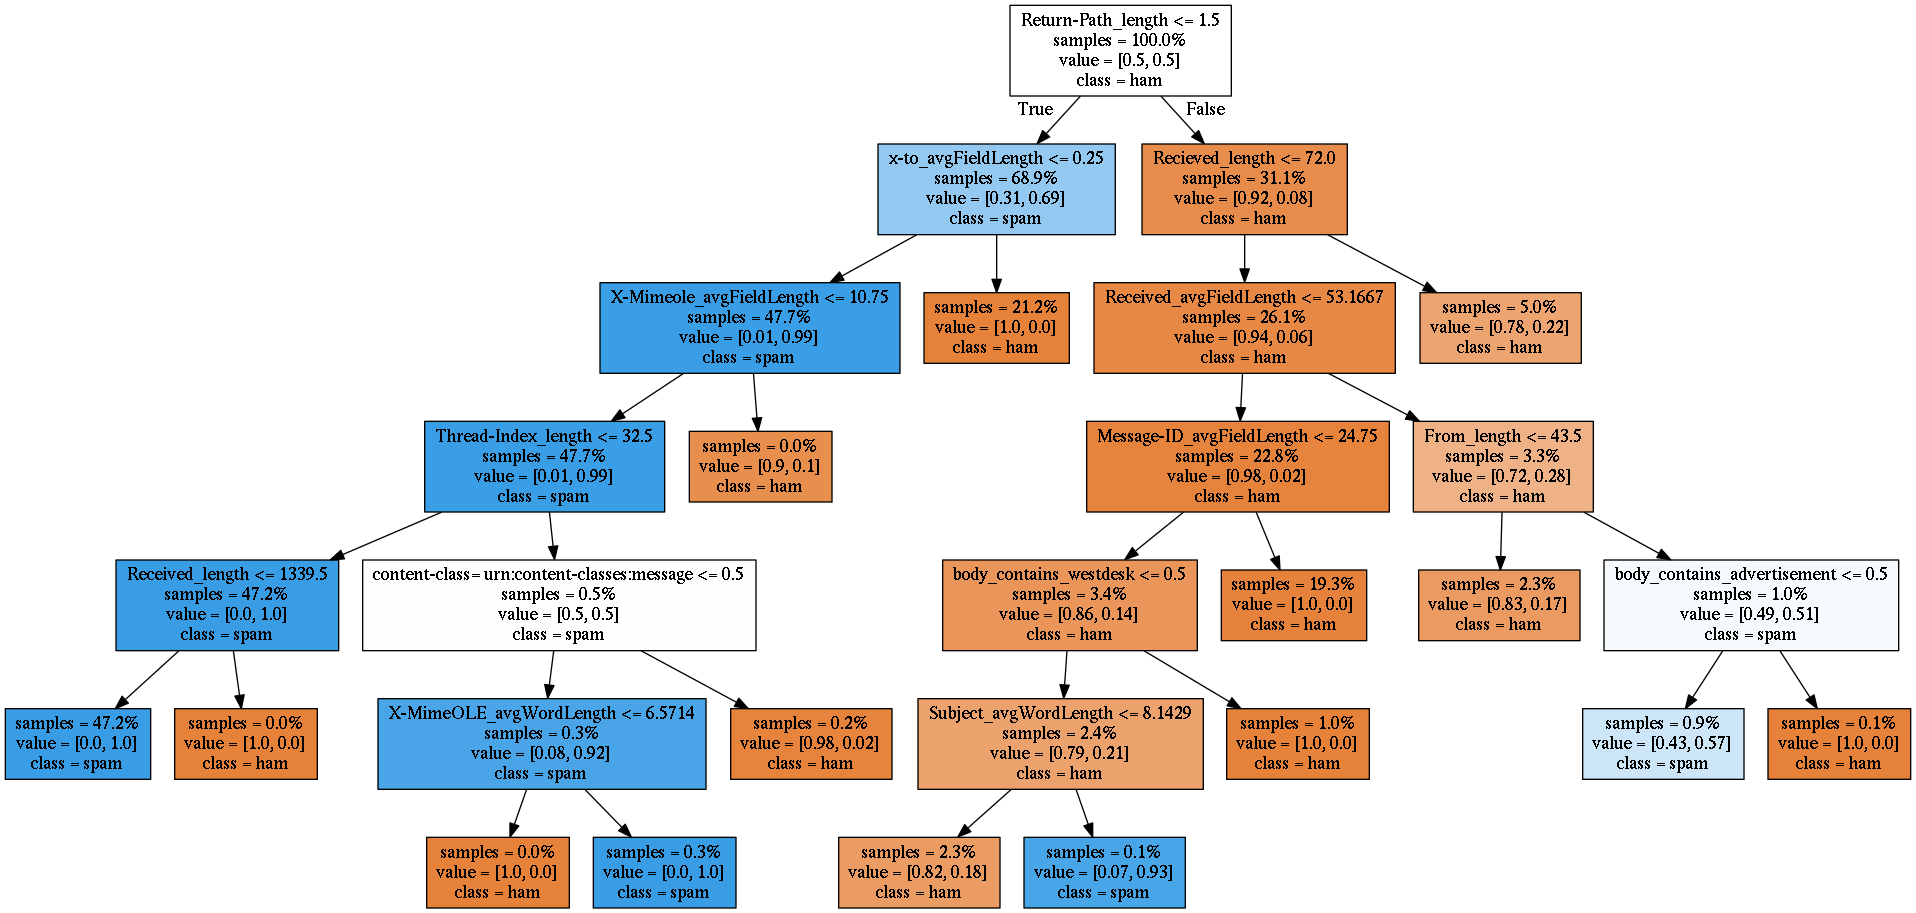
\includegraphics[width=1.3\textwidth]{tree.png}}
	\caption{Árbol de decisión similar con un score un poco menor (pero que es mucho más lindo a la vista).}
\end{figure}

\subsection{Naive Bayes}

Se prueba usar el modelo de Bernoulli usado en sklearn en las variables booleanas del modelo. El único hiperparámetro para elegir es \( \alpha \), el nivel de ``smoothing'' and se le hace a la entrada.

Adicionalmente, los features se separaron en 5 subconjuntos:
\begin{itemize}
	\item \textbf{Existente} Los features \texttt{*\_exists}, que dicen si un campo del header existe o no.
	\item \textbf{Header features} Los features que dan información sobre estos campos.
	\item \textbf{Categorization} Los features que dicen qué valores toman algunos campos.
	\item \textbf{Word bag} Que dicen si cada palabra apareció o no en el mail.
	\item \textbf{Binary} Todos los features binarios, eso es \( \text{Existente} \cup \text{Word Bag} \).
\end{itemize}

Se corrió el estimador de Naive Bayes usando estos subconjuntos de features y diferentes \( \alpha \) y se midió el accuracy de los resultados.

\begin{figure}
	\centerline{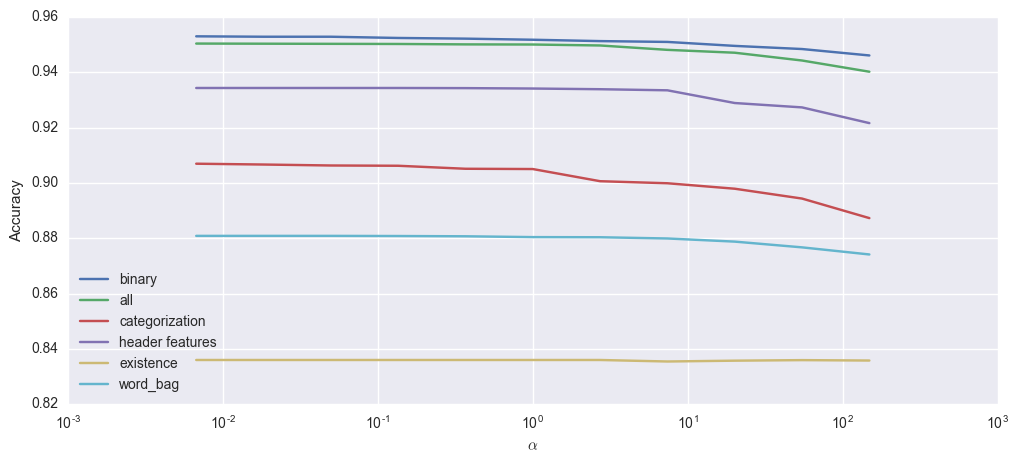
\includegraphics[width=1.3\textwidth]{figures/bayes.png}}
	\caption{Accuracy de los experimentos}
\end{figure}

Se puede ver que el categorizador que usa features binarios suele ser el mejor, y que el accuracy sube cuando baja el smoothing (aunque cuando \( \alpha = 0 \) el accuracy se vuelve particularmente malo). Como de cualquier manera la diferencia es mínima, tomamos \( \alpha = 1 \) y usamos todos los features.

\subsection{K Nearest Neighbors}

Otro estimador que se usó para intentar inferir si un mail es spam o no es el de \textbf{K nearest neighbors}, que decide si un punto forma parte de cada categoría dependiendo de la cantidad o la distancia de puntos de cada categoríá entre los \( K \) que estén a menor distancia Euclideana (u otra medida de distancia).

Dado que hay una gran cantidad de posibles combinaciones para \( K \), y que no se sabe si el mejor estimador usa mayoría absoluta o la suma de las distnacias, se hizo un \textbf{Grid Search} para buscar el valor óptimo de estos parámetros.

\begin{center}
\begin{tabular}{c c c c}
	\toprule
	\textbf{Pesos} & \textbf{K} & \textbf{Avg.\ score} & \textbf{Std.\ score} \\
	\midrule
	uniform & 3 & 0.91765 & 0.00451 \\
	distance & 3 & 0.92062 & 0.00408 \\
	uniform & 5 & 0.90988 & 0.00276 \\
	distance & 5 & 0.91778 & 0.00214 \\
	uniform & 7 & 0.90815 & 0.00134 \\
	distance & 7 & 0.91679 & 0.00048 \\
	\bottomrule
\end{tabular}
\end{center}

Se puede ver que, antiintuitivamente, el méþodo da mejor cuando se toman menos vecinos pero se mide por distancia.

También se intentó hacer una normalización normal a los features, que centra cada componente a uno que tenga media \( \mu = 0 \) y varianza \( \sigma^2 = 0 \).

\[
	f' = \frac{f - \mu_f}{\sigma_f} \; (\forall f \in \text{Features})
\]

De esta manera se le puede dar aproximadamente el mismo peso a cada uno de los features en los métodos. Esto se puede ver en la diferencia con el método anterior.

\subsection{Nearest Centroid}

Esta es una alternative a \textbf{K Nearest Neighbors} donde cada clase se representa por una solo centroide. Aunque parecía tentadora debido a la nula cantidad de parámetros posibles, este método dio un accuracy promedio abismal de \( 0.471 \). Por esta razón no se incluye en el resto de los análisis.

\subsection{Support Vector Machines}

Se usaron \textbf{Support Vector Machines}, que intentan buscar el hiperplano que mejor separa el espacio en dos conjuntos lo más diferentes posibles. Debido a la funcionalidad de este clasificador, se noemalizaron los features de la misma maenra que en la sección de \textbf{K Nearest Neighbors}.

Los tres parámetros importantes de SVM lineal (cuando no se usa el truco de los kernels) son \textbf{C}, que mide la penalidad de un error, \textbf{penalty} decide qué norma usar para medirlo, y \textbf{loss}, que elige una función para normalizar. En los casos donde se usa squared hinge elegimos usar optimización primal contra dual, ya que tenemos una cantidad de samples mucho mayor a la cantidad de features\cite{ngcs229}.

\begin{center}
\begin{tabular}{r c l c c}
	\toprule
	\textbf{C} & \textbf{Penalty} & \textbf{Loss} & \textbf{Avg.\ score} & \textbf{Std.\ score} \\
	\midrule
	0.01 & l1 & squared hinge & 0.97864 & 0.00310 \\
	0.01 & l2 & squared hinge & 0.98519 & 0.00052 \\
	0.01 & l2 & hinge & 0.98506 & 0.00227 \\
	0.1 & l1 & squared hinge & 0.98556 & 0.00181 \\
	0.1 & l2 & squared hinge & 0.98284 & 0.00114 \\
	0.1 & l2 & hinge & 0.98284 & 0.00106 \\
	1 & l1 & squared hinge & 0.98296 & 0.00160 \\
	1 & l2 & squared hinge & 0.98136 & 0.00114 \\
	1 & l2 & hinge & 0.97840 & 0.00251 \\
	10 & l1 & squared hinge & 0.98259 & 0.00297 \\
	10 & l2 & squared hinge & 0.98198 & 0.00149 \\
	10 & l2 & hinge & 0.97901 & 0.00274 \\
	100 & l1 & squared hinge & 0.98296 & 0.00181 \\
	100 & l2 & squared hinge & 0.98160 & 0.00155 \\
	100 & l2 & hinge & 0.97901 & 0.00274 \\
	\bottomrule
\end{tabular}
\end{center}

Se puede ver que los mejores puntajes se dieron cuando se minimiza \textbf{C}, y que la función cuadrática de pérdida (squared hinge) es un poco mejor que la cuadrada que se usa en los kernels lineales. Además, cuando se usa esta función, usar la norma \(l2\) suele dar un mejor resultado que con la norma \(l1\).

\section{Reducción de Dimensionalidad}

\section{Resultados}

\section{Discusión}

\section{Bibliografía}

\begin{thebibliography}{9}

\bibitem{forman2010}
	George Forman \\
	Apples-to-Apples in Cross-Validation Studies: Pitfalls in Classifier Performance Measurement \\
	Hewlett Packard Labs \\
	DOI 10.1.1.186.8880	

\bibitem{ngcs229}
    Andrew Ng \\
	CS229 Lecture Notes \\
	\url{http://cs229.stanford.edu/notes/cs229-notes3.pdf}

\end{thebibliography}

\end{document}
